\section{Introduction}
\label{sec:introduction}
% User-supplied conceptual artwork; original pixels retained for visual fidelity.
% Editable reconstruction and untouched reference page: pairselect_graphical_overview.drawio.
% Curve geometry is illustrative, not a new experimental result.
\begin{figure}[!t]
\centering
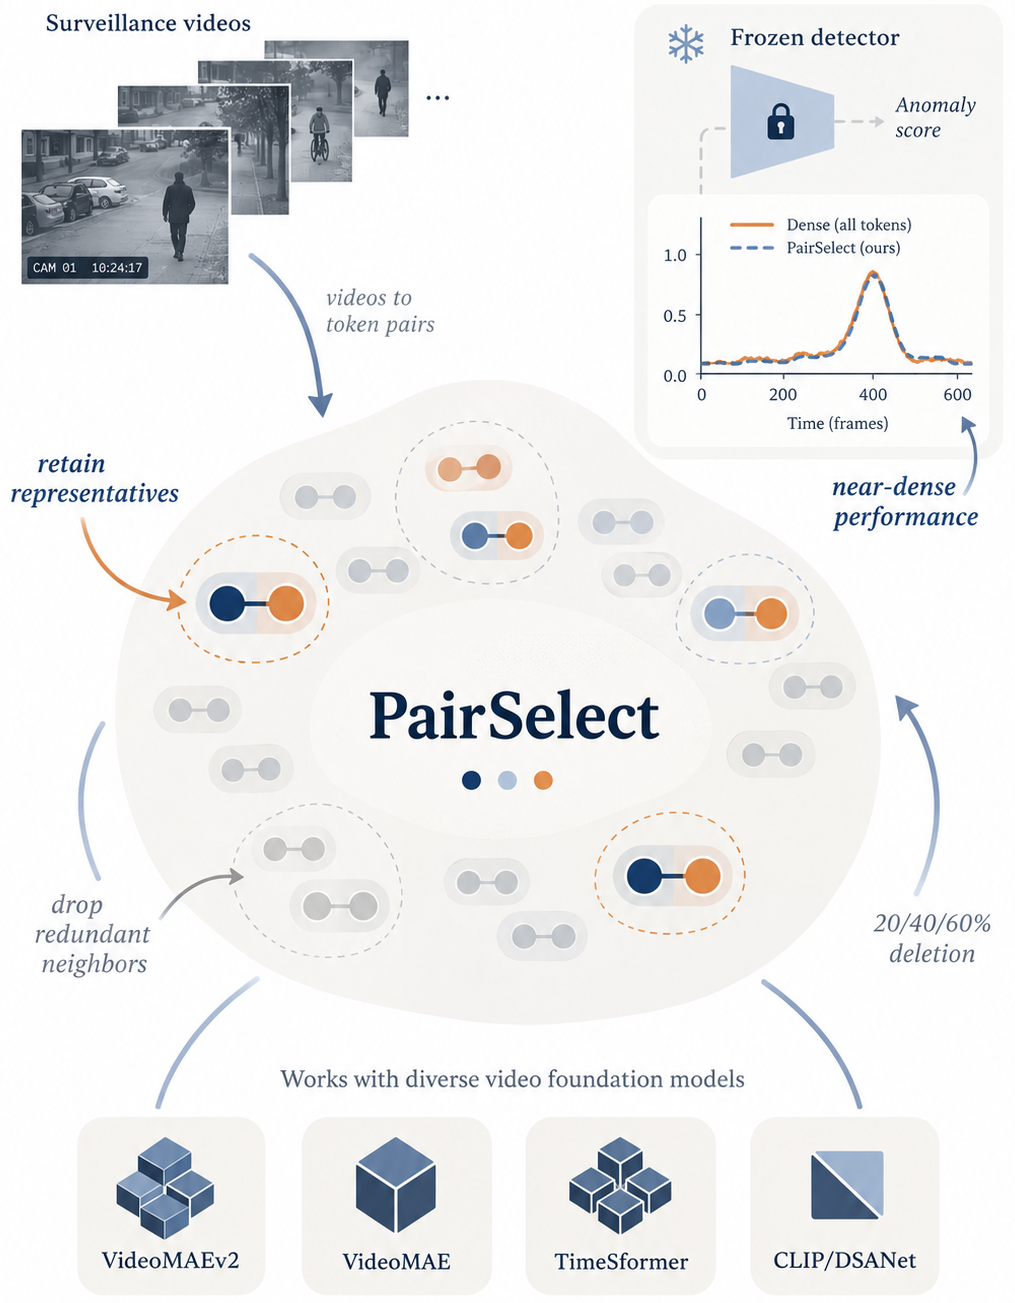
\includegraphics[width=\columnwidth]{figures/pairselect_graphical_overview.png}
\caption{Conceptual overview of \method{}: local representative selection at three deletion budgets with frozen detection across four systems. Score curves are schematic, not measured results.}
\label{fig:concept}
\end{figure}

% Full-width framework figure, updated from the user-approved draw.io.
% PNG is a 2x native render (3072 x 1728), cropped at canvas y=864
% to omit its baked-in caption. The LaTeX caption below is unchanged.
\begin{figure*}[!t]
\centering
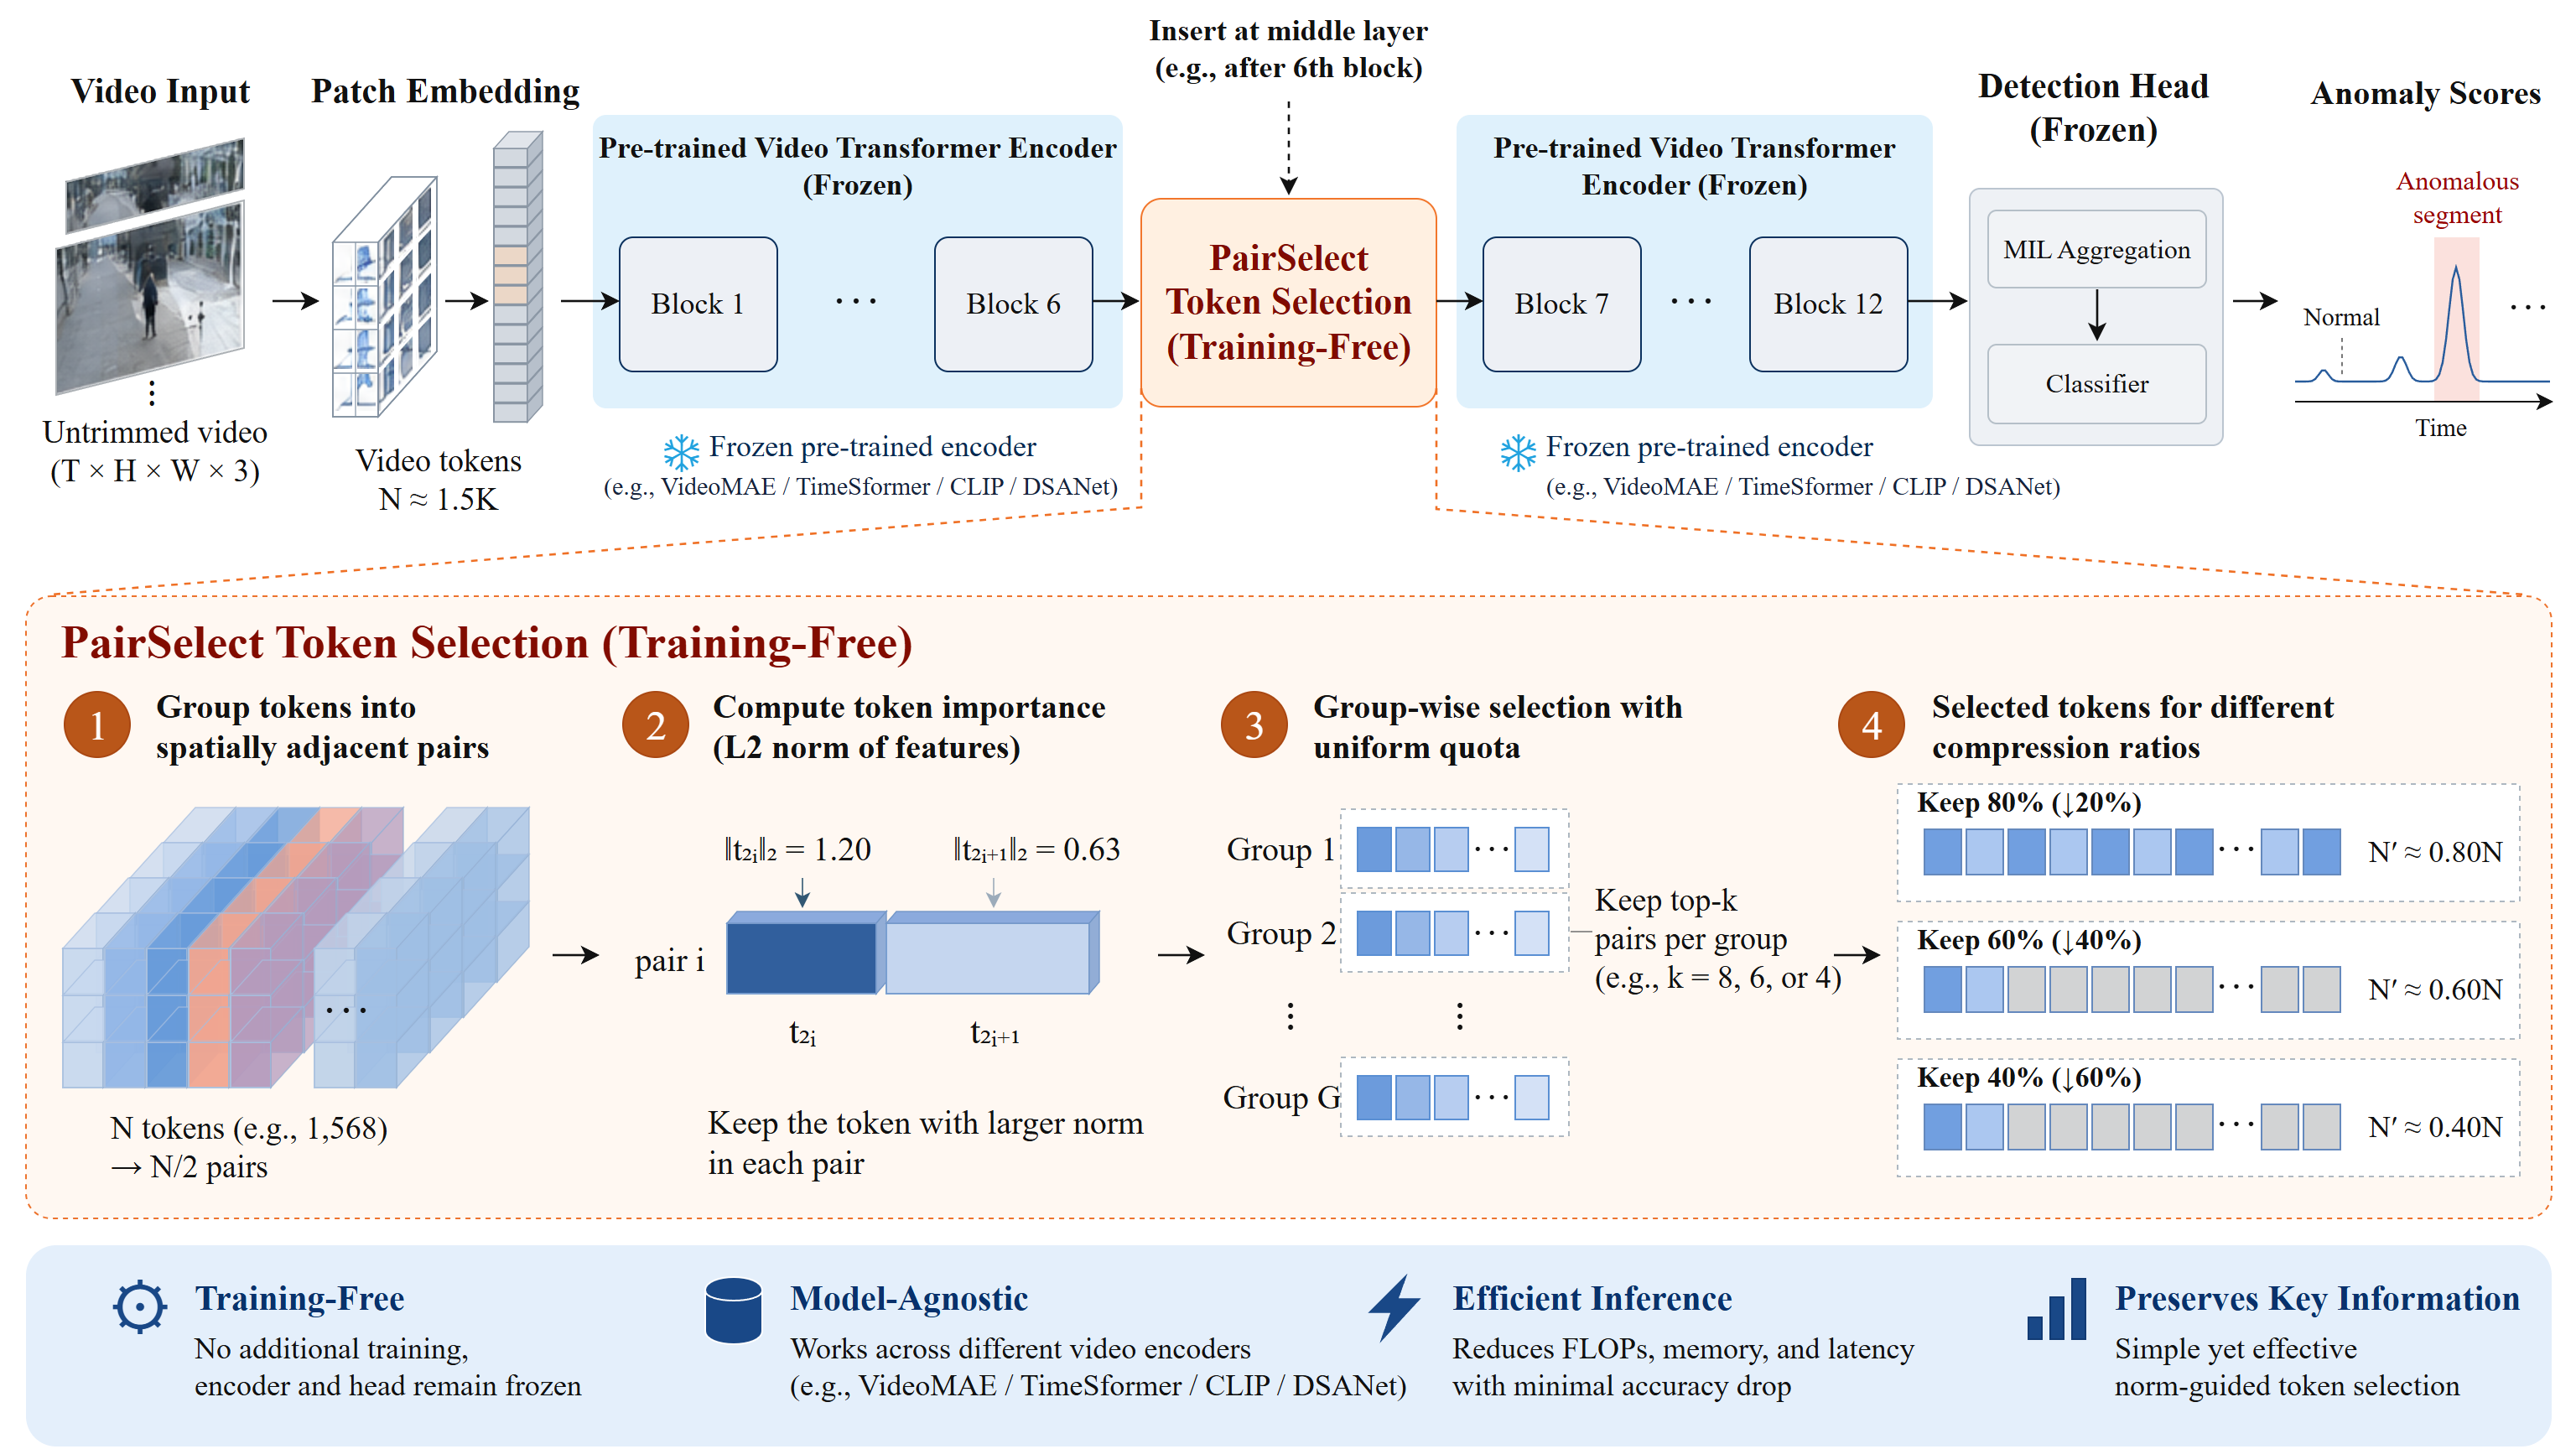
\includegraphics[width=\textwidth]{figures/pairselect_framework.png}
\caption{Overview of \method{}. Six dense blocks contextualize all tokens before local, magnitude-guided selection reduces the input to blocks 7--12. Group quotas control pair-member selection; divided attention retains complete spatial trajectories. The four systems reuse their original temporal sampling and detector weights; CLIP applies pair selection per image and preserves CLS.}
\label{fig:overview}
\end{figure*}

Video anomaly detection faces an asymmetric computational problem: unusual events are scarce, yet the system must process long stretches of ordinary activity to find them. Weakly supervised video anomaly detection (WSVAD) learns from video-level labels without knowing which snippets contain anomalies~\cite{sultani2018real,tian2021rtfm}. Contemporary systems combine pretrained visual representations with temporal detectors, from dual-memory models~\cite{zhou2023urdmu} to CLIP-based semantic alignment~\cite{wu2024vadclip,yin2026learning}. Their representations differ, but they share a deployment question: can an existing detector use less encoding computation without another training cycle?

Reducing the number of sampled clips also changes the temporal observations available to the detector. We instead preserve the original sampling schedule and reduce computation inside the visual encoder. \emph{The rarity of anomalous events does not imply that every internal token carries unique information.} Video redundancy supports masked pretraining~\cite{tong2022videomae,wang2023videomaev2}, while token sampling and merging demonstrate opportunities to process fewer representations~\cite{fayyaz2022ats,bolya2023tome}. This suggests allowing every token to participate in early contextualization, then continuing with locally selected representatives.

We propose \method{}, a non-mixing token selection operator for frozen WSVAD systems (Figs.~\ref{fig:concept} and~\ref{fig:overview}). Local pairing defines where candidates compete, group quotas distribute the budget, and activation magnitude determines member priority. Selected vectors are gathered without averaging. The same principle applies to video-patch representations and CLIP image patches; divided space--time attention instead selects complete spatial trajectories. Neither the visual encoder nor the detector is retrained after insertion or when the budget changes.

Our evaluation jointly covers four systems: VideoMAEv2-B, VideoMAE-B, and TimeSformer-B with their respective UR-DMU heads, and CLIP ViT-B/16 with the published DSANet weights. DSANet is a recent high-performance, state-of-the-art-level WSVAD system~\cite{yin2026learning}, making this a test of transfer across both visual representations and detector designs. We contribute the local selection rule, its architecture-aware application, and a complete three-budget quality--efficiency study on two datasets. At 40\% nominal deletion, most configurations retain near-dense quality; 60\% deletion offers greater encoder throughput with generally mild quality costs.
